\documentclass[14pt, a4paper]{extreport}

\usepackage[margin=3cm]{geometry}
\usepackage[T2A]{fontenc}
\usepackage[utf8]{inputenc}
\usepackage[main=bulgarian, english]{babel}
\usepackage{graphicx}

\usepackage{xcolor}
\definecolor{comment}{HTML}{7F848E}
\definecolor{keyword}{HTML}{88aaee}
\definecolor{function}{HTML}{bb66ff}
\definecolor{type}{HTML}{2266ff}
\definecolor{string}{HTML}{d0ac55}
\definecolor{directive}{HTML}{966440}
\definecolor{background-code}{rgb}{0.95,0.95,0.95}
\definecolor{background-shell}{rgb}{0.3,0.3,0.3}

\usepackage{hyperref}
\hypersetup{
    colorlinks=true,
    allcolors=blue,
    % linkcolor=darkgray,
    % urlcolor=blue,
    % citecolor=blue,
    pdftitle={Diploma},
    pdfpagemode=FullScreen,
}

\usepackage[acronym, toc]{glossaries}
\makenoidxglossaries
\newacronym{ansi}{ANSI}{American National Standards Institute}
\newacronym{api}{API}{Application Programming Interface}
\newacronym{ci}{CI}{Continuous Integration}
\newacronym{crud}{CRUD}{Create, Read, Update, Delete}
\newacronym{db}{DB}{Database}
\newacronym{gnu}{GNU}{GNU's not Unix!}
\newacronym{graphql}{GraphQL}{Graph Query Language}
\newacronym{http}{HTTP}{Hyper Text Transfer Protocol}
\newacronym{json}{JSON}{JavaScript Object Notation}
% \newacronym{os}{OS}{}
% \newacronym{raii}{RAII}{Resource Acquisition Is Initialization}
\newacronym{rest}{REST}{Representational State Transfer}
\newacronym{yaml}{YAML}{YAML Ain't Markup Language}
\newacronym{oop}{ООП}{Обектно-Ориентирано Програмиране}
% \item[cpm] - C/C++ Package Manager (използвано вместо ``програмата'')
% \item СУП - Система за Управление на Пакети (Package Manager)

\newcommand{\figref}[1]{(фиг. \ref{#1})}
\newcommand{\lstref}[1]{(списък \ref{#1})}

\usepackage{listings}
\usepackage[scale=.85]{sourcecodepro}
\renewcommand{\lstlistingname}{Списък}
\lstdefinestyle{shell}{
    basicstyle=\ttfamily\small\color{white},
    backgroundcolor=\color{background-shell},
    rulecolor=\color{background-shell},
    language=sh,
    tabsize=4,
    captionpos=b,
    keywordstyle=\color{comment},
    framexleftmargin=6pt,
    framextopmargin=6pt,
    framexbottommargin=6pt,
    frame=ltbr, % framerule=0pt,
    frameround=tttt,
    % commentstyle=\color{codegreen},
    % stringstyle=\color{codepurple},
    % breakatwhitespace=false,
    % breaklines=true,
    % keepspaces=true,
    % showspaces=false,
    % showstringspaces=false,
    % showtabs=false,
}
\lstdefinestyle{cpp}{
    basicstyle=\ttfamily\footnotesize,
    backgroundcolor=\color{background-code},
    rulecolor=\color{background-code},
    language=C++,
    tabsize=4,
    captionpos=b,
    numbers=left,
    numberstyle=\ttfamily\color{gray},
    keywordstyle=\color{keyword}\textbf,
    commentstyle=\color{comment}\textit,
    stringstyle=\color{string},
    directivestyle=\color{directive}\textit,
    xleftmargin=20pt,
    framexleftmargin=26pt,
    framextopmargin=6pt,
    framexbottommargin=6pt,
    frame=ltbr, % framerule=0pt,
    frameround=tttt,
    % breakatwhitespace=false,
    % breaklines=true,
    % keepspaces=true,
    % showspaces=false,
    % showstringspaces=false,
    % showtabs=false,
}
\lstdefinestyle{json}{
    basicstyle=\ttfamily\footnotesize,
    backgroundcolor=\color{background-code},
    rulecolor=\color{background-code},
    % language=JSON,    % no such language apparently!
    tabsize=4,
    captionpos=b,
    numbers=left,
    numberstyle=\ttfamily\color{gray},
    commentstyle=\color{comment}\textit,
    morestring=[b]",
    morestring=[d]',
    stringstyle=\color{type},
    xleftmargin=20pt,
    framexleftmargin=26pt,
    framextopmargin=6pt,
    framexbottommargin=6pt,
    frame=ltbr, % framerule=0pt,
    frameround=tttt,
    % breakatwhitespace=false,
    % breaklines=true,
    % keepspaces=true,
    % showspaces=false,
    % showstringspaces=false,
    % showtabs=false,
}

\usepackage[sorting=none]{biblatex}
\addbibresource{references.bib}

\usepackage{pdfpages}

\usepackage{float}
\usepackage[font=small, skip=5pt]{caption}

\usepackage{array}
\usepackage{adjustbox}
\usepackage{amsfonts}
\usepackage{amsmath}
\usepackage{amssymb}
\usepackage{cancel}


\begin{document}

\graphicspath{ {./images/} }

\begin{titlepage}
	\begin{adjustbox}{tabular=m{3cm} m{14cm}, center}
		% \includegraphics[scale=0.15]{tues_logo_transperent-500x500}
		% &
		% \shortstack{
		% 	\textbf{\small ТЕХНОЛОГИЧНО УЧИЛИЩЕ „ЕЛЕКТРОННИ СИСТЕМИ“} \\
		% 	\textbf{\small към ТЕХНИЧЕСКИ УНИВЕРСИТЕТ - СОФИЯ}
		% }
	\end{adjustbox}

    % \begin{wrapfigure}{l}{.15\textwidth}
    %     % \centering
    %     \includegraphics[scale=0.15]{tues_logo_transperent-500x500}
    % \end{wrapfigure}

    \begin{center}
        \vspace{4cm}
        \textbf{\Huge КУРСОВА РАБОТА}

        % по професия код 481020 „Системен програмист“

        % специалност код 4810201 „Системно програмиране“
    
        \vspace{3cm}
        {\LARGE Тема: Симулатор на орбити}
    
        \vspace{5cm}
        % \begin{tabular*}{.8\textwidth}{@{\extracolsep{\fill}} l r }
        %     \textbf{Дипломант:} & \textbf{Научен ръководител:} \\
        %      Ясен Ефремов & Валентин Върбанов
        % \end{tabular*}
        \textbf{Изготвил:} \\
        Ясен Ефремов
    
        \vfill
        СОФИЯ \\
        2024 г.
    \end{center}
\end{titlepage}



\printnoidxglossary[type=\acronymtype, title={Използвани съкращения}, sort=def]


% \chapter*{Увод}

В днешно време хората използват по-голямо количество софтуер от когато и да
било. Като започнем от ежедневно употребяваните програми, а именно уеб
браузърът, редакторите за документи, софтуерът за обработка на изображения,
видео и аудио, и стигнем чак до видеоигрите. Средностатистическият потребител,
е свикнал да си набавя всякакъв вид софтуер като просто потърси за него в
интернет пространството, намери достатъчно достоверно изглеждаща уеб страница,
от която да го свали, и изтегли приложението под формата на автоматизиран
инсталатор (файлове с разширение .msi, .deb, .dmg) или директно изпълним файл
(файлове с разширение .exe). Този подход обаче има недостатъци, най-големите от
които са удобството и сигурността. На всеки се е случвало при инсталирането на
даден софтуер да се изгуби из множеството уеб страници, опитващи се да те
заблудят като рекламират различни продукти или дори поставят фалшиви бутони за
инсталация, водещи към непознати подозрителни сайтове. Освен че по този начин си
губи времето, потребителят също така е изложен и на риск от заразяване със
зловреден софтуер. Един от начините да се избегне всичко това е използването на
система за управление на пакети (package manager). Тя позволява намирането,
инсталирането и актуализирането на софтуер безопасно под формата на пакети,
валидирани от истински хора и съхранявани в сигурни хранилища. Това има
множество предимства - унифицира се начина на работа със софтуерни пакети,
улеснява се работата на потребителя и се намалява риска от злонамерени действия
срещу него. Популярни примери за системи за управление на пакети са winget за
Windows, apt за Ubuntu Linux и homebrew за MacOS.

Системите за управление на пакети обаче могат да бъдат полезни и за самите
разработчици на софтуер. Една от основните им функции е да знаят от какви други
програми (библиотеки) е зависима дадена програма и съответно да управляват тези
зависимости. Големите софтуерни проекти са съставени от множество модули, които
зависят едни от други. Освен това всеки модул има различни версии, всяка от
които може да предоставя различни функционалности. Някои модули зависят от точно
определена версия на други модули. Така се създава една доста заплетена мрежа от
зависимости, която изисква постоянна поддръжка. Ако трябваше програмистът ръчно
да се грижи за всичко това, работата му щеше да се увеличи значително. За щастие
почти всеки език за програмиране в днешно време има своя система за управление
на пакети. Езикът Python има системата pip, езикът JavaScript има системата npm,
езикът Java има две такива системи - maven и gradle, и дори Rust, език за
системно програмиране, сравним със C и C++, има своя система, наречена cargo.
За жалост едни от езиците, които нямат общоприета система са именно C и C++. Има
опити да се направи такава, но въпреки това голяма част от програмистите
предпочитат да се грижат за зависимостите на проектите си ръчно. Една от
причините за това е факта, че и двата езика са създадени преди повече от 30
години и съответно следват по-различни практики от съвременните езици за
програмиране. Въпреки това C и C++ продължават да бъдат развивани и до ден
днешен, като и двата езика постепенно се сдобиват с нови по-модерни
функционалности.

Текущият проект цели реализирането на система за управление на пакети за
програмните езици C и C++. Самата система е написана на C и C++, като предоставя
конзолен потребителски интерфейс, посредством който могат да се инсталират и
премахват пакети под формата на хранилища, взети от онлайн платформата GitHub.
Системата също така позволява управление на зависимостите на даден пакет, както
и създаването на изцяло нови пакети, описани чрез файловия формат
\acrshort{json}.

% \addcontentsline{toc}{chapter}{Увод}
\graphicspath{ {./chapter1/images/} }

\chapter{Увод}


\section{Описание и идея на проекта}

Идеята на проекта е да представлява много опростена версия на програми като
STK (Systems Tool Kit) и GMAT (General Mission Analysis Tool), които позволяват
планиране и симулиране на космически мисии. Тези програми са изключително
сложни, затова текущият проект се стреми да реализира само задаването,
пресмятането и рисуването на орбитата на сателит, обикалящ около идеално
сферично тяло. Крайната програма трябва да представлява графично Desktop
приложение с полета за задаване на параметрите на симулацията и прозорец
показващ как би изглеждала симулираната орбита.


\section{Цел и задачи на разработката}

Основните функционалности на програмата са разпространението на сателита в
зададена орбита и визуализирането на получените данни.



% \section{Структура на документацията}


% \tableofcontents


\graphicspath{ {./chapter2/images/} }

\chapter{Преглед на предметната област}


\section{Основни дефиниции, концепции и алгоритми, които ще бъдат използвани}

Всяка орбита може да бъде описана напълно от 6 стойности. Има два начина на описание:

\begin{itemize}
	\item Чрез 6-те орбитални елемента, задаващи Кеплерова орбита:
	\begin{itemize}
		\item Ексцентрицитет \( e \)
		\item Голяма полуос \( a \)
		\item Наклон на орбитата \( i \) 
		\item Дължината на възходящия връх \( \Omega \)
		\item Параметър на перихелия \( \omega \)
		\item Истинска аномалия \( \nu \)
	\end{itemize}
	\item Чрез вектори на орбиталното състояние, задаващи позицията и скоростта на тялото:
	\begin{itemize}
		\item Вектор на позицията \( \vec{r} = \left( r_x, r_y, r_z \right) \in \mathbb{R}^3 \)
		\item Вектор на скоростта \( \vec{v} = \left( v_x, v_y, v_z \right) \in \mathbb{R}^3 \)
	\end{itemize}
\end{itemize}

Самата орбита представлява конично сечение, като обикаляното тяло се намира в единия от неговите фокуси.

За простота приемаме, че обикаляното тяло е идеална сфера с маса  и гравитационна константа .

Разполагаме с диференциалните уравнения, описващи начина, по който се променя скоростта и позицията на сателита с времето:

\begin{align*}
	\frac{d\vec{v}}{dt} &= -\frac{MG}{|\vec{r}|^2}\frac{\vec{r}}{|\vec{r}|} \\
	\frac{d\vec{r}}{dt} &= \vec{v}
\end{align*}

Да намерим аналитично решение на такива уравнения е прекалено трудно (дори често невъзможно). Можем обаче да намерим тяхно числено решение. Това означава, че разполагаме с начални стойности за търсената функция.
След това избираме дискретна времева стъпка  и с нейна помощ намираме следващата стойност на функцията. Така получаваме апроксимация на търсената функция. Този метод се нарича метод на Ойлер. При него обаче се натрупва грешка. Тя може да бъде минимизирана чрез методите на Верле или на Рунге-Кута.


% \section{Дефиниране на проблеми и сложност на поставената задача}




% \section{Подходи и методи за решаване на поставените проблеми}




\section{Потребителски изисквания и качествени изисквания}

Програмата трябва да предоставя графичен потребителски интерфейс (GUI), чрез
който да могат да се задават начални стойности на симулацията.


\graphicspath{ {./chapter3/images/} }

\chapter{Проектиране}


\section{Обща архитектура – ООП дизайн}

При разработката на проекта бяха използвани съвременни ООП практики като
полиморфични йерархии от класове и Factory шаблонът.


\section{Диаграми}

\begin{figure}[h]
	\centering
	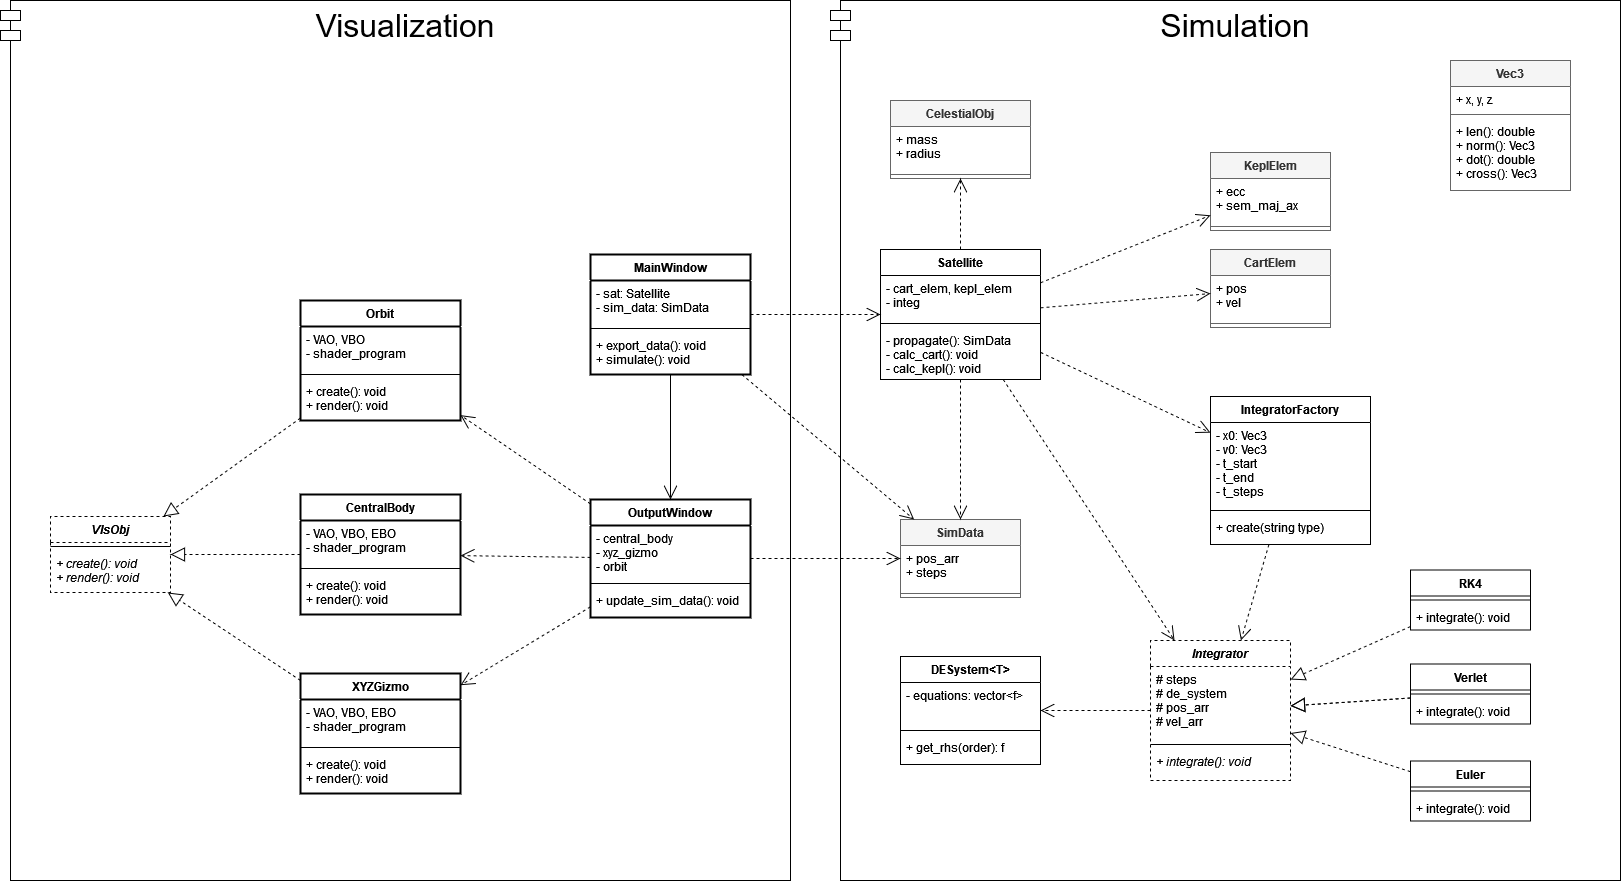
\includegraphics[width=\textwidth]{structure.png}
	\caption{UML диаграма на структурата на проекта}
\end{figure}


\graphicspath{ {./chapter4/images/} }

\chapter{Реализация, тестване}


\section{Реализация на класове}

Ключови за проекта са класовете \texttt{Satellite} и \texttt{Integrator}. Класът
\texttt{Integrator} е абстрактен и бива използван за реализацията на методите на
Ойлер, Верле и Рунге-Кута. Класът \texttt{Satellite} съдържа описанието на
орбитата си и може да превръща Кеплеровите елементи във вектори на състоянието и
обратно.


\section{Управление на паметта и алгоритми. Оптимизации.}

Местата, на които бе необходимо ръчно управление на паметта, са най-вече
масивите от генерирани данни от симулацията. Те се управляват от класът
\texttt{Integrator}, като се освобождават в неговия деструктор според
принципа RAII.

При симулацията най-важни са алгоритмите за пресмятане на позицията и скоростта
на сателита, както и тези за превръщане на Кеплеровите елементи в Декартови и
обратното \cite{cart_to_kepl} \cite{kepl_to_cart} \cite{classical_orb_elem}. Те
са оптимизирани да работят със стойности без размерност, което
увеличава тяхната точност. Размерността се пренася изцяло от следните три
константи:

\begin{align*}
	R_0 &= R_E \\
	V_0 &= \sqrt{\frac{M_E G}{R_E}} \\
	T_0 &= \frac{R_0}{V_0}
\end{align*}

След нормиране на векторите на позицията и скоростта получаваме следните
диференциални уравнения

\begin{align*}
	\vec{r} &= R_0 \vec{\rho} \Rightarrow \frac{d\vec{r}}{dt} = \cancel{\frac{R_0}{T_0}} \frac{d\vec{\rho}}{d\tau} = \cancel{V_0} \vec{u} \Rightarrow \frac{d\vec{\rho}}{d\tau} = \vec{u} \\
	\vec{v} &= V_0 \vec{u} \Rightarrow \frac{d\vec{v}}{dt} = \cancel{\frac{V_0}{T_0}} \frac{d\vec{u}}{d\tau} = - \cancel{\frac{M_E G}{R_0^3}} \frac{\vec{\rho}}{\left\lvert \rho \right\rvert^3 } \Rightarrow \frac{d\vec{u}}{d\tau} = -\frac{\vec{\rho}}{\left\lvert \rho \right\rvert^3 } \\
	t &= T_0 \tau
\end{align*}


\section{Планиране, описание и създаване на тестови сценарии}

За тестване на кода бе използвана библиотеката GoogleTest. Класът
\texttt{Integrator} и неговите наследници бяха тествани чрез т.н. Fixture,
който позволява преизползване на инициализирани променливи в множество тестове


\graphicspath{ {./chapter4/images/} }

\chapter{Заключение}


\section{Обобщение на изпълнението на началните цели}

Основните цели на проекта, а именно
\begin{itemize}
	\item Задаване и симулиране на орбитата на сателит
	\item Записване на симулираните параметри в текстов файл
	\item Рисуване на обикаляното тяло
	\item Рисуване на орбитата на сателита
\end{itemize}
бяха изпълнени, с което се предоставя работеща начална версия на софтуера.


\section{Насоки за бъдещо развитие и усъвършенстване}

Към проекта могат да бъдат добавени функционалности, които да позволяват
симулиране на повече от един сателит, планиране и изпълнение на мисии, съставени
от множество маневри, запазване и зареждане на симулацията във и от файл и
други.

% \chapter*{Заключение}

Настоящата дипломна работа реализира базов вариант на система за управление на
пакети за програмните езици C и C++. Системата бе написана на C++, като е
достъпна за платформите Linux и Windows. Тя предоставя конзолен потребителски
интерфейс, посредством който могат да бъдат изпълнени команди, позволяващи
инсталирането, премахването, изброяването, създаването и синхронизирането на
софтуерни пакети. Като регистър за съхранение на пакетите бе използвана
платформата GitHub. Системата предоставя механизъм за автоматично управление на
зависимостите на пакетите посредством символични връзки (symlinks). Други
допълнителни функционалности са воденето на диагностични записки и показването
на анимирани индикатори за напредък по време на изпълнението на програмата.

Възможностите за бъдещо развитие на проекта са многобройни: следващата голяма
цел би била разработката на собствен регистър за съхранение на пакети,
предоставящ специално разработени точки за достъп (endpoints), позволяващи
по-лесно сдобиване с кода на пакетите и техните зависимости; други цели са
автоматична компилация на кода при теглене на пакетите, поддръжка за други build
системи освен CMake (например Meson и Bazel) и много допълнителни команди,
улесняващи потребителя - команда за търсене на пакети, команда за актуализация
на вече инсталирани пакети, команда за автоматично публикуване на новосъздадени
пакети и други.

% \addcontentsline{toc}{chapter}{Заключение}


\tableofcontents


\printbibliography


\end{document}
